\documentclass{article}
\usepackage{tikz}
\usetikzlibrary{arrows,shapes}
 
\begin{document}

%% you can give labels to the nodes, and can refer to them later.  
 
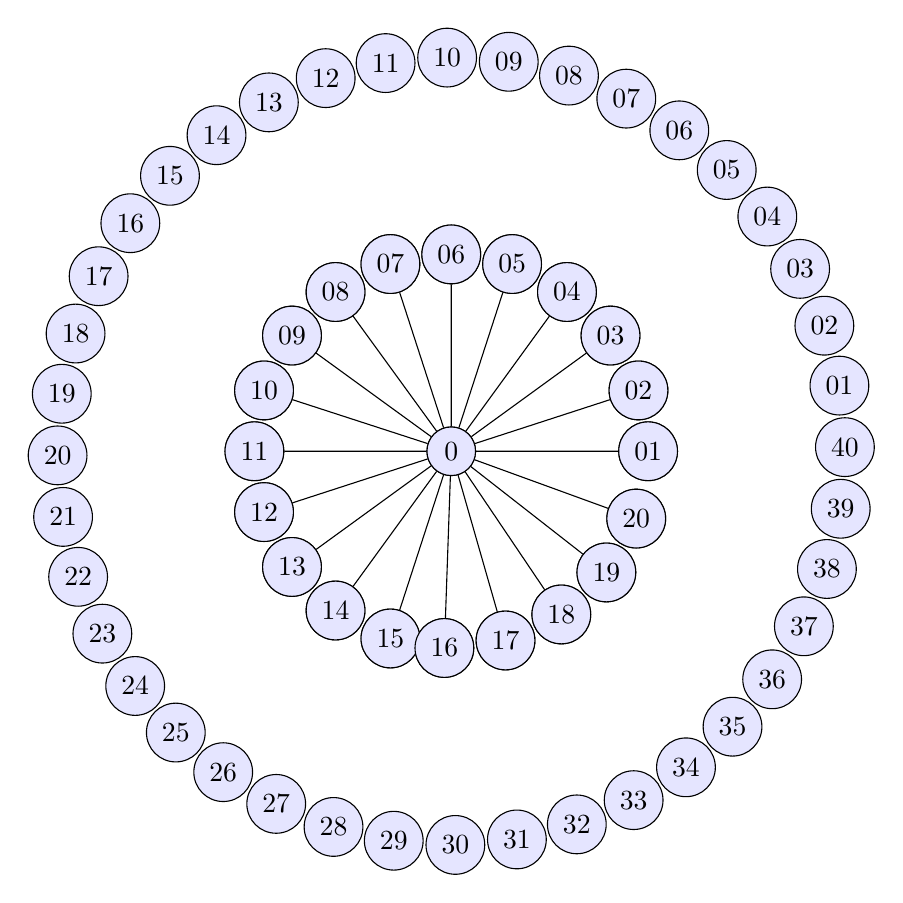
\begin{tikzpicture}[scale=2.5]
\tikzstyle{every node}=[draw,shape=circle,radius=2.2cm,fill=blue!10];
\path (0:0cm) node (0) {$0$};
\path (0:1cm) node (1) {$01$};
\path (18:1cm) node (2) {$02$};
\path (36:1cm) node (3) {$03$};
\path (54:1cm) node (4) {$04$};
\path (72:1cm) node (5) {$05$};
\path (90:1cm) node (6) {$06$};
\path (108:1cm) node (7) {$07$};
\path (126:1cm) node (8) {$08$};
\path (144:1cm) node (9) {$09$};
\path (162:1cm) node (10) {$10$};
\path (180:1cm) node (11) {$11$};
\path (198:1cm) node (12) {$12$};
\path (216:1cm) node (13) {$13$};
\path (234:1cm) node (14) {$14$};
\path (252:1cm) node (15) {$15$};
\path (268:1cm) node (16) {$16$};
\path (286:1cm) node (17) {$17$};
\path (304:1cm) node (18) {$18$};
\path (322:1cm) node (19) {$19$};
\path (340:1cm) node (20) {$20$};

\path (0:0cm) node (0) {$0$};
\path (0:1cm) node (1) {$01$};
\path (18:1cm) node (2) {$02$};
\path (36:1cm) node (3) {$03$};
\path (54:1cm) node (4) {$04$};
\path (72:1cm) node (5) {$05$};
\path (90:1cm) node (6) {$06$};
\path (108:1cm) node (7) {$07$};
\path (126:1cm) node (8) {$08$};
\path (144:1cm) node (9) {$09$};
\path (162:1cm) node (10) {$10$};
\path (180:1cm) node (11) {$11$};
\path (198:1cm) node (12) {$12$};
\path (216:1cm) node (13) {$13$};
\path (234:1cm) node (14) {$14$};
\path (252:1cm) node (15) {$15$};
\path (268:1cm) node (16) {$16$};
\path (286:1cm) node (17) {$17$};
\path (304:1cm) node (18) {$18$};
\path (322:1cm) node (19) {$19$};
\path (340:1cm) node (20) {$20$};

\foreach \i in {1,...,9}
{

   \path (\i*9+0.6:2cm) node (123) {0\i};
   %\fill (X\i) circle (.31cm);
}
\foreach \i in {10,...,40}
{

   \path (\i*9+0.6:2cm) node (123) {\i};
   %\fill (X\i) circle (.31cm);
}


\draw (0) -- (1)
(0) -- (2)
(0) -- (3)
(0) -- (4)
(0) -- (5)
(0) -- (6)
(0) -- (7)
(0) -- (8)
(0) -- (9)
(0) -- (10)
(0) -- (11)
(0) -- (12)
(0) -- (13)
(0) -- (14)
(0) -- (15)
(0) -- (16)
(0) -- (17)
(0) -- (18)
(0) -- (19)
(0) -- (20)
;
\end{tikzpicture}


\end{document}